\newpage
\appendix

\section{Implementation}
\label{sec:implementation}

Wollok language is developed on top of Xtext\footnote{http://www.eclipse.org/Xtext/}, which is an Eclipse\footnote{https://www.eclipse.org/home/index.php} project aiming to provide a set of tools for language development. It’s what is now called a Language Workbench\footnote{http://martinfowler.com/articles/languageWorkbench.html}.
This allows us to get rid of all the necessary effort required to build a language from scratch, like coding a parser or lexical analyser. But also it also gives us seamless integration with the Eclipse IDE. Being a language workbench means that it already addresses concerns we already mentioned would be really useful for new programmers, like: content assist (\figref{codetemplates.png}), quick fixes (\figref{quickfix.png}), cross-references searches, etc.

\subsection{Backend}

Given our Wollok grammar in a pseudo BNF form, Xtext then provides us with the parser and AST represented as Java ECore models part of the EMF project\footnote{http://www.eclipse.org/modeling/emf/}. Then there are several options for the backend when working with XText. The three most classics are: (1) to generate code through templates, (2) to generate Java code through an specific API, (3) to make your own way with a Java interpreter.

All three have their pro’s and con’s. For Wollok we decided to go on with option 3, meaning that Wollok is a fully interpreted language, with its backend being a Java application.
We prioritized simplicity for developers, \eg avoiding java code generation, and also full control of the execution in backend. 

The price for this is that we’ve lost the \emph{out-of-the-box} type checking code generation through API would give us, and also the XText debugger.
Although the first one wouldn’t have applied anyway without some effort for
customizing XText, since Wollok is a completely type annotations-free language,
and XText bases its default type system on some sort of annotations.

For the debugger, we have just developed a custom eclipse plugin which already
provides around 80\% of any industrial type language debugger.

This debugger can even be abstracted into a reusable XText component for any other interpreted language.

\subsection{Type System}

XText type system is currently implemented on top of XSemantics\footnote{http://xsemantics.sourceforge.net}, a DSL for writing rules for XText languages. XSemantics is itself made with XText.
This allows us to develop our type system in a declarative way. The type system can be seen in action in \figref{check-messageSending.png}.

\subsection{Development}

As with any software testing is really important, but unlike any common application, testing a language has many difficulties.
Wollok mixes up several techniques for testing its development.
Part of the interpreter logic is being tested with unit test in JUnit. While for some other aspects that are more tied up with xtext and eclipse components we are using XPect\footnote{http://www.xpect-tests.org}, a unit and integration-testing framework for Xtext languages.
XPect is in turn also developed as an XText language.
It provides a declarative way to annotate Wollok programs with expected
behaviour like validator’s errors/warnings, or code completions,  etc.

\section{The Wollok Software}
\seclabel{wollokSoftware}

\subsection{Features}

The Wollok Development Environment provides a number of feature for a rich programming experience, like:

\begin{itemize}
 \item Text editor with syntax highlight.
 \item Content assist
 \item Code templates
 \item Auto-build and checks along with quick fixes.
 \item Problems and warning (markers) tracking both in editors, files, and view problems. See section \secref{ChecksAndValidations}
 \item Run and debug integration with eclipse launcher framework. Providing a debug perspective integration, as well as a console.
 \item Code navigation and cross-references searches working almost as an explicitly typed language.
 \item UI Wizards for creating projects other Wollok entities.
\end{itemize}


\begin{figure}[ht]
    \centering
	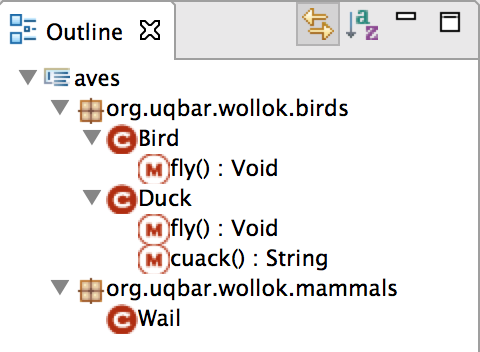
\includegraphics[scale=0.5]{images/wollok-paper-outline.png}
    \caption{Outline View: This view shows the structure of the file.}
    \label{fig:outline.png}
\end{figure}

\begin{figure}[ht]
    \centering
	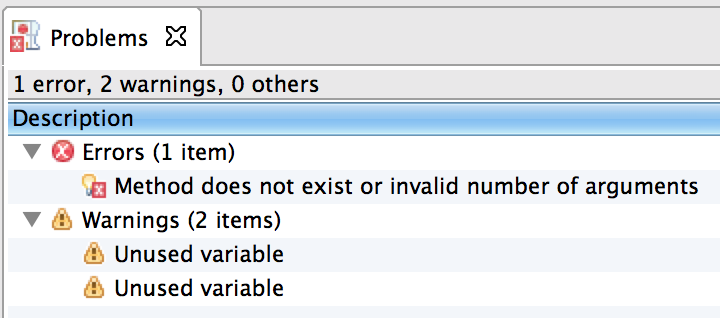
\includegraphics[scale=0.5]{images/wollok-paper-check-problemsview.png}
    \caption{Problems View: shows the different problems detected by the IDE }
    \label{fig:problemsview.png}
\end{figure}

\begin{figure}[ht]
    \centering
	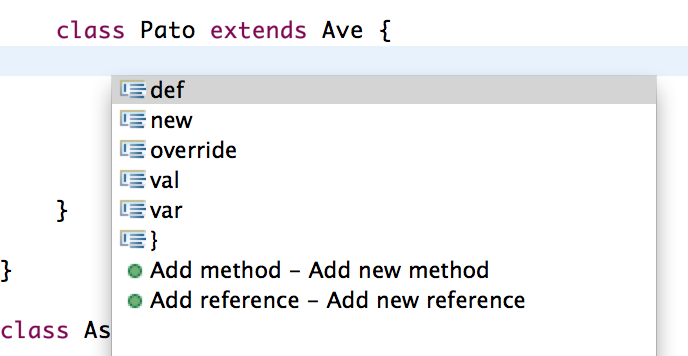
\includegraphics[scale=0.5]{images/wollok-paper-codetemplates.png}
    \caption{Code Assist: code templates for easy edition}
    \label{fig:codetemplates.png}
\end{figure}

\begin{figure}[ht]
    \centering
	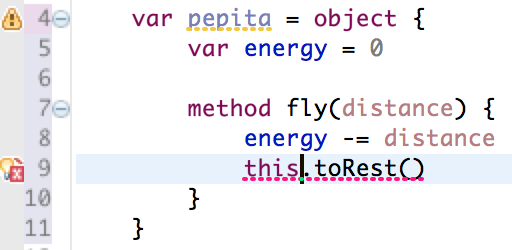
\includegraphics[scale=0.5]{images/wollok-paper-check-noMethodOnThis.png}
    \caption{Detection of an error on sending a message to \emph{this}}
    \label{fig:check-noMethodOnThis.png}
\end{figure}

\begin{figure}[ht]
    \centering
	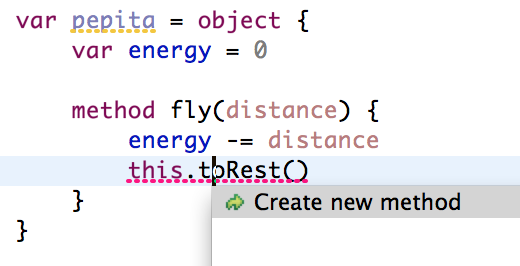
\includegraphics[scale=0.5]{images/wollok-paper-quickfix.png}
    \caption{Quick fix tool for common errors and mistakes}
    \label{fig:quickfix.png}
\end{figure}

\begin{figure}[ht]
    \centering
	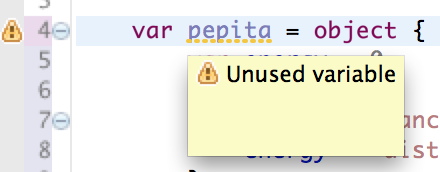
\includegraphics[scale=0.5]{images/wollok-paper-check-unusedVariable.png}
    \caption{Detection of unused variables}
    \label{fig:check-unusedVariable.png}
\end{figure}

\begin{figure}[ht]
    \centering
	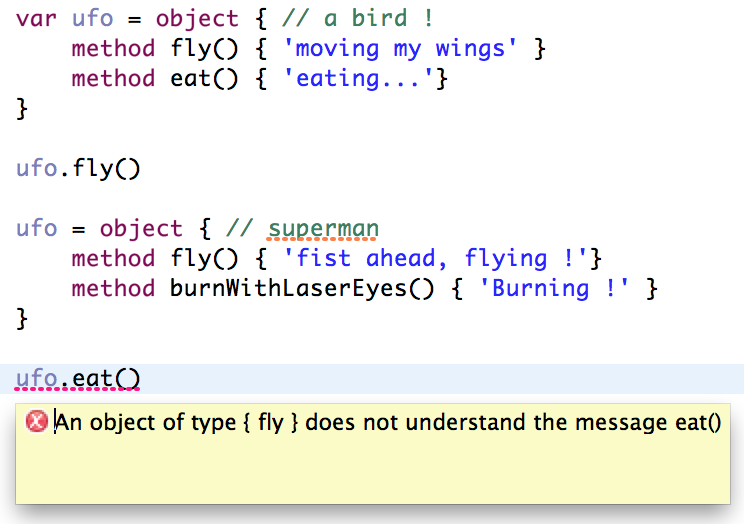
\includegraphics[scale=0.5]{images/wollok-paper-check-messageSending.png}
    \caption{Type system in action, detecting not defined method for the message sent}
    \label{fig:check-messageSending.png}
\end{figure}


\subsection{Software availability}

Wollok is open-sourced and distributed under LGPLv3 License\footnote{http://www.gnu.org/copyleft/lgpl.html}.
Source code and documentation can be found in Bitbucket (\url{https://bitbucket.org/uqbar-project/wollok}) 
And mirrored at Github (\url{https://github.com/uqbar-project/wollok})

\section{Examples of Checks and validations}
\seclabel{ChecksAndValidations}

All the results of the checking and the validation of the program is shown in one integrated view, it is called \emph{Problems}. The figure \figref{problemsview.png} shows a view of this feature. 
There are different types of problems, because these checks and validations are not only used to show type errors or syntax errors, but also to encourage some properties of the program we consider as main topics in the learning process of an OO language.

Here is a list of all the validations and checks the tool supports, and a
brief reason why they are useful while teaching object oriented programming.

\begin{itemize}
  \item \textbf{Syntax Errors}: this category involves all the errors detected
  by the parser and the lexical analyser of the language.
  \item \textbf{Style Errors}: this category is useful to teach good practices and to start to talk about code quality, reuse and code sharing.
	\begin{itemize}
		\item \textit{Case in Names}: respecting the difference case conventions for
		names (\eg using \textit{camelCase} starting with lower case for variables,
		using camel case starting with upper case for classes).
		\item \textit{Order and grouping}: inside the definition of an object or class the internal references are declared first, then the constructors and finally the methods.
		\item \textit{Modularization}: the classes can only be defined in a library and not in the main program.		
		\item \textit{Duplicated references}: it is impossible to declare a reference
		using a name already used. This encourage the idea of not having shadowing and
		improves the readability of the program.
	\end{itemize}
  \item \textbf{References resolution problems}: this errors are useful to detect and avoid references to undeclared variables and also errors in the sending of messages.
  
	\begin{itemize}
	  \item \textit{Undeclared references}: from local variables, parameters or internal fields of objects and classes.
	  \item \textit{Undefined constructors}: checking for the number and type of the parameters.
	  \item \textit{Messages to this}: sending messages to this is a special case, here we can check the existence of the correct method by the number and type of the arguments, even without using type inference.
	\end{itemize}
	
  \item \textbf{Reference usage}: these errors are useful for the detection of
  erroneous or \textit{dead code} (\eg unused variables or references, sending
  messages to never assigned variables, using variables instead of values, existence of the overridden method.

  \item \textbf{Type Errors}: the errors are useful for the validation of the compatibility between the references, its possible types, and the messages sent to them, this is performed by the type system and its inferer (\eg message sending, assignation of variables).
\end{itemize}


